\section{Introduction}
\label{sec:introduction}

% state the learning objective 
\paragraph{} The objective of this laboratory assignment is to study a circuit composed of eleven branches and eight nodes, arranged in four independant meshes,
 as detailed bellow. This circuit has seven resistences, numbered from $R_1$ trough $R_7$, dependant current and volatage sources, $V_C$ and $I_B$ respectively,
 and independant current and voltage sources, $V_A$ and $I_D$ respectively.
The study of the circuit will be subdivided in two major steps. In Section 2 we will analyse the circuit using the Mesh and Node Analysis. In Section 3 the circuit is going to be simulated with Ngspice, and we will compare the results of that simulation with the ones obtained in Section 2.
Finally, the Conclusions of this assignment are detailed in Section 4.

\begin{figure}[h] \centering
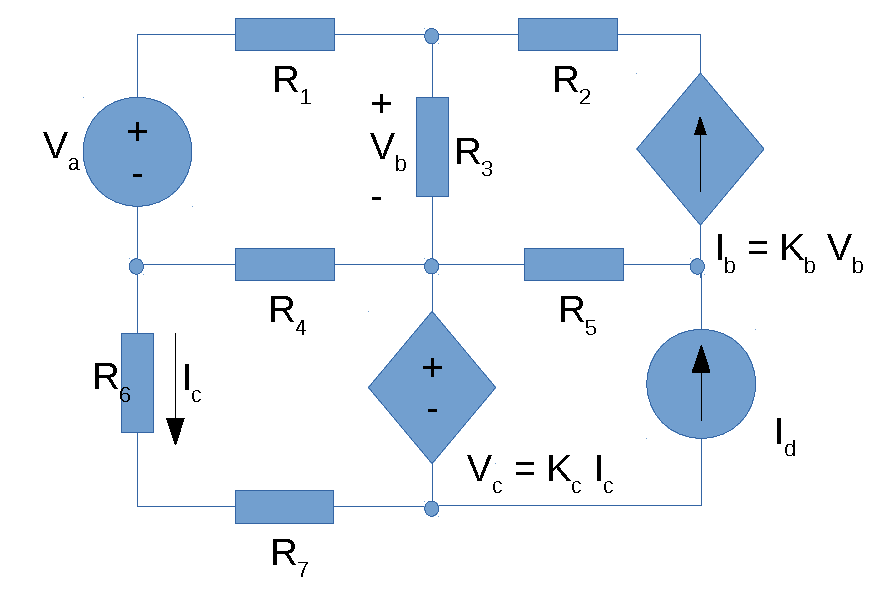
\includegraphics[width=0.5\linewidth]{circuit.pdf}
\caption{Circuit to be analyzed in the laboratory assignment.}
\label{fig:rc}
\end{figure}

